\documentclass{article}
\usepackage[margin=1in, top = .8in, left=.8in]{geometry}
\usepackage{comment}
\usepackage{amsmath, amssymb}
\usepackage{framed}
\usepackage{enumerate}
\usepackage{comment}
\usepackage{tikz,pgfplots}
\usepgfplotslibrary{fillbetween}
\pgfplotsset{compat=1.15}
\usepackage[hyphens]{url}

\begin{document}

 \begin{center}
    \large \textbf{Homework 4}
\end{center}
    %\item[\textbf{Week 4}]
            \begin{enumerate}
                 \item Determine the intervals on which the following function is increasing/decreasing.  $$f(x)=2x^3+3x^2-120x+60$$
                 \item What are the local maximum and local minimum values for the function $f(x) = e^{(x^5-x^4-2x^3+x^2-1)}$? Note that a local extreme value is a $y$-value, not an $x$-value.
                \item Find the absolute minimum of the function 
                $$f(x) = x^2\ln{x}$$
                Start by paying attention to the domain of the function. Show all of your work, and include a complete argument that an absolute minimum occurs at the critical value you find.
                \item The purpose of this question is to practice using logarithms to find critical values. Since $\ln{x}$ is an increasing function, the critical values of any function $f(x)$ occur at the same place as the critical values of $\ln{(f(x))}$. In this question you'll find the critical values of a function without using logarithms, then you'll find the critical values using logarithms. Assume for these questions that the domain is $0 < p < 1$. Note that you are asked for a critical value, so your answer should be a value for $p$, not $L(p)$.
                \begin{itemize}
                    \item Find the critical values of the function $L(p) = p^x(1-p)^{1-x}$ by finding where $L'(p) = 0$.
                    \item Find the critical values of the function $\ln{(L(p))}$. Confirm you get the same result is in the previous part.
                \end{itemize} 
                \item Find the critical values of the function $\displaystyle \ell(\vec{x}:\lambda) = \prod_{k=1}^{n} \frac{\lambda^{x_k}e^{-\lambda}}{x_k!}$. Here $\vec{x}=(x_1,x_2,\dots,x_n)$ is a list of $n$ constants.
                
 




                \item Find the most general antiderivative of each of the following functions. You have not learned any formal rules yet for antidifferentiation, so solve these problems by guessing/checking/revising. Check all of your answers by differentiating (don't forget the chain rule!)
                    \begin{enumerate}
                        \item $\displaystyle g_1(x) = \pi x^4-ex^3+\sqrt{x}+2\pi e + \frac{2}{ex}$
                        \item $g_2(x) = x\cdot e^{x^2}$
                        \item $g_3(x) = \frac{\ln{x}}{x}$
                        \item $g_4(x)= \frac{\textnormal{acorn}(x)}{\textnormal{tree}(x)} +\textnormal{flop}(\textnormal{tree}(x))\cdot \textnormal{acorn}(x)$.  The following information will be needed.
                        \begin{itemize}
                            \item $\frac{d}{dx}[\textnormal{flip}(x)] = \textnormal{flop}(x)$
                            \item $\frac{d}{dx}[\textnormal{flop}(x)] = \textnormal{tree}(x)$
                            \item $\frac{d}{dx}[\textnormal{tree}(x)] = \textnormal{acorn}(x)$
                        \end{itemize}
                    \end{enumerate}
 
 
                                \item Approximate the region graphed here using a Riemann sum with five rectangles.  You can choose left-hand endpoints, right-hand endpoints, or midpoints; just make your choice clear.
                \begin{center}
                    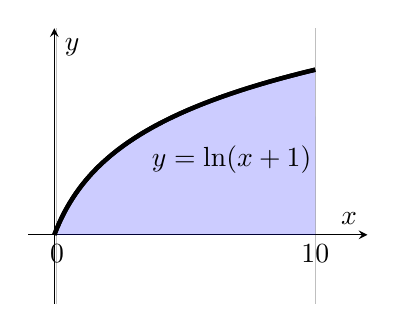
\begin{tikzpicture}
                        \begin{axis}[
   	                    xmin=-1, xmax=12,
    	                ymin=-1, ymax=3,
	                    xtick={0.1,10},  
	                    xticklabels={0,10},
	                    ytick=\empty,
	                    major tick length={0},
	                    line width=1pt,
 	                    axis lines=center, height=2 in, grid=major, ylabel=$y$, xlabel=$x$
	                    ]
                        \addplot [ultra thick, samples=100, domain=0:10] {ln(x+1)} node [pos=0.35, below right] {$y=\ln(x+1)$};
                        \addplot [name path = f1,ultra thick, samples=9, domain=0:10, samples = 100] {ln(1+x)};
                            \path[name path=axisf1] (axis cs:0,0) -- (axis cs:10,0);
                        \addplot [
                        thick,
                        color=blue,
                        fill=blue, 
                        fill opacity=0.20, samples=100
                        ]
                        fill between[
                        of=f1 and axisf1
                        ];
                        \end{axis}
                    \end{tikzpicture}
                \end{center}

                        \item For each of the following, approximate the area under the function $f(x)$ using $n$ rectangles of equal width and right-hand endpoints. These problems relate closely to several problems you did in previous work.
                            \begin{enumerate}
                                \item $\displaystyle f(x) = \frac{1}{5}x+4$ on the interval $[0,10]$ and $n=10$  
                                \item $\displaystyle  f(x) = x^2-4x+5$ on the interval $[1, 5]$ and $n=8$ \\ %\textcolor{red}{(the summation problem is $\displaystyle \sum_{j=1}^{8} \frac{1}{2}\left[\left(1+\frac{j}{2} \right)^2 -4\left( 1+ \frac{j}{2}\right) + 5\right]$)}
                            \end{enumerate}
                \item Consider the function $f(x) = x^2-x+1$ on the interval $[0,4]$.  Find the general formula for the Riemann sum with $n$ rectangles, using $\Delta x = \frac{b-a}{n}$ and righthand endpoints.  Then, take the limit to find the exact area between $f(x)$ and the $x$-axis from $x=0$ to $x=4$. This problem relates closely to a problem you already solved in previous work. \\
               % \textcolor{red}{Faan Tone, I put the following summation problem in Week 1 under the same instructions as the two summations mentioned just above. $\displaystyle \sum_{j=1}^{n} \frac{4}{n}\left[ \left(\frac{j}{n}\right)^2 - \frac{j}{n} + 1 \right]$}
                \item Find the value of $\displaystyle \int_{0}^{3} \sqrt{9-x^2}\,dx$ by graphing the appropriate region and calculating the area using basic geometry facts.
                \item If $\displaystyle \int_a^b f(x)\,dx = c$, what does $\displaystyle \int_a^b 77f(x)\,dx$ equal? Explain.
                \item If $\displaystyle \int_a^b f(x)\,dx = c$, and $\displaystyle \int_a^b g(x)\,dx = d$, what does $\displaystyle \int_a^b f(x)+g(x)\,dx$ equal? Explain.
                \item If $a < b < c$,  $\displaystyle \int_a^c f(x)\,dx = 15$, and $\displaystyle \int_c^b f(x)\,dx = 23$, then what does $\displaystyle \int_a^b f(x)\,dx$ equal?
                    \item Suppose I tell you that the definite integral
$\displaystyle \int_0^x f(t)\,dt = e^{x^3}$.
\begin{enumerate}
    \item Find $\displaystyle \int_0^2 f(t) \,dt$.
    \item Find $\displaystyle \int_1^3 f(t)\,dt$.
    \item Find $\displaystyle \int_{-1}^1 f(t)\,dt$.
\end{enumerate}
                \end{enumerate}

\end{document}